% cSpell: disable
\def\qualifigsepigogd{.1mm}
\section{Deep Learning for MRI reconstruction}

\begin{frame}[plain,c]
    %\frametitle{A first slide}

    \begin{center}
        \color{DarkBlue}
    \Huge \thesection. \insertsection
    \end{center}

\end{frame}

% XXX have visual aid in all equations
\begin{frame}{Model agnostic learning}
    % reframing the problem as supervised learning
    % no knowledge of the physics imposed in the model
    % The first use of DL for MRI reconstruction is to actually throw away most of what we just saw:\footfullcite{Zhu2018}
    Let's throw away all we know:\footfullcite{Zhu2018}
    \begin{equation*}
        f_{\thetab}(\measurements) = \imageb
    \end{equation*}
    \begin{tikzpicture}[overlay,remember picture,>=stealth,nodes={align=left,inner ysep=1pt},<-]
        % For "kspace"
        \onslide<2->{
        \path (kspace.south) ++ (0,-4em) node[anchor=south east,color=amber!87] (exp_kspace){
            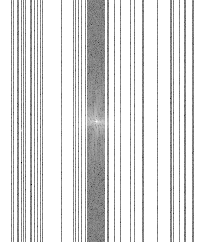
\includegraphics[width=0.07\textwidth]{Figures/intro_figures/kspace_mri.png} \textbf{kspace}};
        \draw [color=amber!87](kspace.south) |- ([xshift=-0.3ex,color=amber]exp_kspace.south west);
        }
        % For "image"
        \onslide<3->{
        \path (image.south) ++ (0, -4em) node[anchor=south west,color=blue!87] (exp_image){
            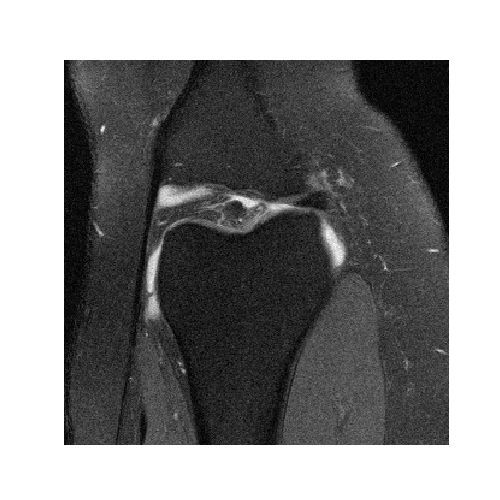
\includegraphics[width=0.1\textwidth,trim=0 3.3em 0 0,clip]{Figures/dl_mri_figures/gt_knee.png} \textbf{image}};
        \draw [color=blue!87](image.south) |- ([xshift=-0.3ex,color=blue]exp_image.south east);
    }
    \end{tikzpicture}

    \onslide<4->{
        \vspace{3em}
        Cons:
    \begin{itemize}
        \item Not taking advantage of our knowledge of the physics
        \item No scaling
    \end{itemize}
    }
\end{frame}

\begin{frame}{Single domain learning}
    % Use the backward operator as a basis for the restoration model
    % We actually have access to the backward operator $\mathcal{A}^H$, the inverse FT composed with the sensitivity maps.

    Let's use $\mathcal{A}^H$ to build a more informed model \alt<2->{in the image space}{in the k-space}:
    \begin{equation*}
        \alt<1>{\adjointop}{}f_{\thetab}(
            \tikzmarknode{aliased_image}{\alt<2->{\adjointop}{}\measurements}
        ) = \imageb
    \end{equation*}

    \begin{tikzpicture}[overlay,remember picture,>=stealth,nodes={align=left,inner ysep=1pt},<-]
        % For image
        \path (image.south) ++ (0, -4em) node[anchor=south west,color=blue!87] (exp_image){
            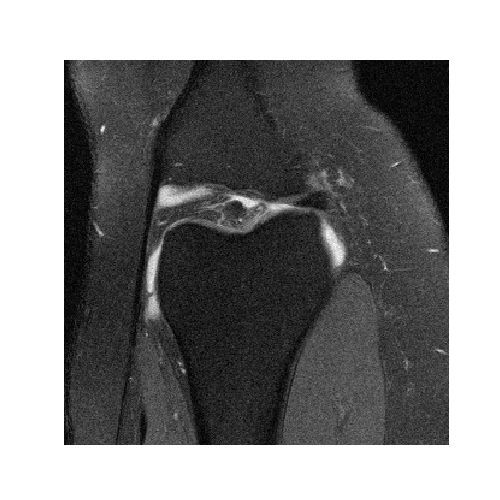
\includegraphics[width=0.1\textwidth,trim=0 3.3em 0 0,clip]{Figures/dl_mri_figures/gt_knee.png} \textbf{image}};
        \draw [color=blue!87](image.south) |- ([xshift=-0.3ex,color=blue]exp_image.south east);
        % For kspace
        \onslide<1>{
            \path (kspace.south) ++ (0,-4em) node[anchor=south east,color=amber!87] (exp_kspace){
                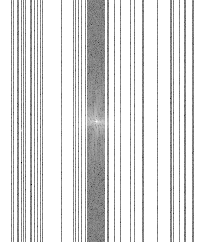
\includegraphics[width=0.07\textwidth]{Figures/intro_figures/kspace_mri.png} \textbf{kspace}};
            \draw [color=amber!87](kspace.south) |- ([xshift=-0.3ex,color=amber]exp_kspace.south west);

        }
        % For aliased image
        \onslide<2>{
        \path (kspace.south) ++ (0, -4em) node[anchor=south east,color=amber!87] (exp_aliased_image){
            \includegraphics[width=0.1\textwidth,trim=0 3.3em 0 0,clip]{Figures/dl_mri_figures/zfilled_recon_af4.png}\textbf{aliased image}};
        \draw [color=amber!87](kspace.south) |- ([xshift=-0.3ex,color=amber]exp_aliased_image.south west);
        }
    \end{tikzpicture}

\end{frame}

\begin{frame}{Unrolled models - 1}
    % recovery algorithm and corresponding computation graph
    % show on second slice unrolled computation graph
    We can mix the 2 single domain approaches, using the principled \textbf{optimization algorithm unrolling} method.\footfullcite{Gregor2010}

    \alt<5->{}{A graph representation of ISTA:}
    \begin{columns}[totalwidth=\textwidth]
        \begin{column}[]{0.3\textwidth}

            \begin{equation*}
                \begin{split}
                    \xb_{n+1} &= \highlight{yellow}{$\xb_n - \epsilon_n \mathcal{A}^H\left(\mathcal{A} \xb_n - \ybb\right)$}\\
                    \xb_{n+1} &= \alt<5->{\highlight{blue}{$f_{\thetab_n}\left(\xb_{n+1}\right)$}}{\highlight{blue}{$\operatorname{prox}_{\epsilon_n \mathcal{R}}\left(\xb_{n+1}\right)$}}
                \end{split}
            \end{equation*}

        \end{column}
        \begin{column}[]{0.6\textwidth}
            \only<2-3>{
                \begin{tikzpicture}[font=\scriptsize, node distance=1em,>=stealth]
                    % nodes
                    \node (input) {$\xb_0$};
                    \node (dc) [rounded rectangle, right=of input, draw=yellow!87, fill=yellow!17] {
                    \alt<3>{Data Consistency step~(DC)}{$\cdot - \epsilon_n \mathcal{A}^H\left(\mathcal{A} \cdot - \ybb\right)$}
                    };
                    \node (prox) [rounded rectangle, right=of dc, draw=blue!87, fill=blue!17] {
                        \alt<3>{Proximal step~(Prx)}{$\operatorname{prox}_{\epsilon_n \mathcal{R}}\left(\cdot\right)$}
                    };
                    % arrows linking all 4 nodes
                    \draw [->] (input) -- (dc);
                    \draw [->] (dc) -- (prox);
                    % arrow linking the prox to the dc in a loop fashion
                    \draw [->] (prox.east) -| ($(prox.east)+(0.5em, -2em)$) -| (dc.south);
                \end{tikzpicture}
            }
            \only<4->{
                \begin{tikzpicture}[font=\scriptsize, node distance=1em,>=stealth]
                    \tikzset{
                        position label/.style={
                        below = 0.em,
                        text height = 1.5ex,
                        text depth = 1ex
                        },
                        brace/.style={
                            decoration={brace, mirror},
                            decorate
                        }
                    }
                    % nodes
                    \node (input) {$\xb_0$};
                    \node (dc_1) [rounded rectangle, right=of input, draw=yellow!87, fill=yellow!17] {DC};
                    \node (prox_1) [rounded rectangle, right=of dc_1, draw=blue!87, fill=blue!17] {\alt<5->{$f_{\thetab_1}$}{Prx}};
                    \node (dots) [right=of prox_1] {$\ldots$};
                    \node (dc_2) [rounded rectangle, right=of dots, draw=yellow!87, fill=yellow!17] {DC};
                    \node (prox_2) [rounded rectangle, right=of dc_2, draw=blue!87, fill=blue!17] {\alt<5->{$f_{\thetab_N}$}{Prx}};
                    \node (output) [right=of prox_2] {$\xb_{N}$};
                    \node (whole) [visible on=<6->, fit=(dc_1) (prox_1) (dots) (dc_2) (prox_2), draw, rounded rectangle, inner sep=0.1em] {};
                    \node (whole_exp) [visible on=<6->, below=of whole] {The whole network};
                    % arrows linking all nodes
                    \draw [->] (input) -- (dc_1);
                    \draw [->] (dc_1) -- (prox_1);
                    \draw [->] (prox_1) -- (dots);
                    \draw [->] (dots) -- (dc_2);
                    \draw [->] (dc_2) -- (prox_2);
                    \draw [->] (prox_2) -- (output);
                    % brace
                    \draw<4-5> [brace, line width=0.25mm] ($(dc_1.south west)+(0,-0.25em)$) -- ($(prox_1.south east)+(0,-0.25em)$) node [position label, pos=0.5] {$\times N$};
                    \draw<6-> [line width=0.1em] (whole.south) -- (whole_exp.north);
                \end{tikzpicture}
            }
        \end{column}
    \end{columns}
\end{frame}


\begin{frame}{Unrolled models - 2}
    % first benchmark: different unrolling strategies give different results
    \begin{exampleblock}{Contribution \#1}
        \fullcite{Ramzi2020_benchmark_journal}
    \end{exampleblock}
    % We can build different models depending on the optimization algorithm we unroll, the choice of $f_{\thetab}$ and the number of iterations.
    Different models based on:
    \begin{itemize}
        \item optimization algorithm to unroll
        \item choice of $f_{\thetab}$
        \item $N$
    \end{itemize}
    \pause

    \begin{overprint}


    \onslide<2>
        \vspace{-1em}
        \begin{table}[h]
            % \large
            \centering
            \caption{\textbf{Quantitative results for the fastMRI dataset.} The PSNR is computed over the 200 validation volumes.}
            \label{tab:quanti-fastmri}
            \vspace{-0.5em}
            \begin{tabular}{l|c|c|c|c|c}
            \textbf{Network} & \textbf{Zero-filled} & \textbf{KIKI-net} & \textbf{U-net} & \textbf{Cascade net} & \textbf{PD-net}\footnotemark \\ \hline
            \textbf{PSNR} & 29.61 & 31.38 & 31.78 & 31.97 & \textbf{32.15}
            \end{tabular}%
            \end{table}

        % XXX dk why I need to write the number manually but this needs to change
        % if the footnotes change
        \footnotetext{$^8$\fullcite{Adler2018}}
\end{overprint}



\end{frame}

\begin{frame}
    \def\thefigdim{.205}
    \def\qualifigsep{-6mm}
    \begin{figure}
        \begin{center}\hspace*{-.3cm}
        \begin{tabular}{@{\hspace*{\qualifigsep}}c@{\hspace*{\qualifigsep}}c@{\hspace*{\qualifigsep}}c@{\hspace*{\qualifigsep}}c@{\hspace*{\qualifigsep}}c@{\hspace*{\qualifigsep}}c@{\hspace*{\qualifigsep}}}
        {\textbf{Reference}} & {\textbf{Zero-filled}} & {\textbf{KIKI-net}} & {\textbf{U-net}} & {\textbf{Cascade-net}} & {\textbf{PD-net}} \\
        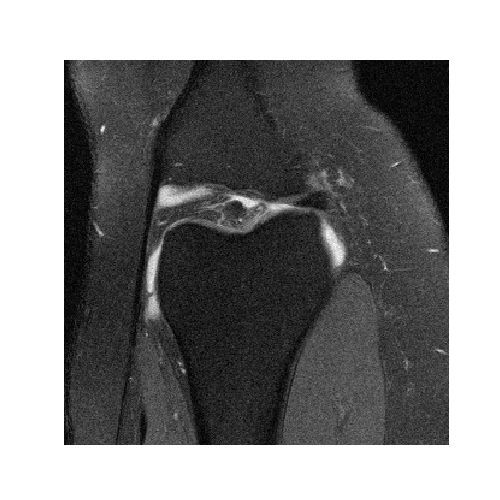
\includegraphics[width=\thefigdim\linewidth]{Figures/dl_mri_figures/bench_figs/image_gt.png}&
        \includegraphics[width=\thefigdim\linewidth]{Figures/dl_mri_figures/bench_figs/zfilled_recon_af4.png}&
        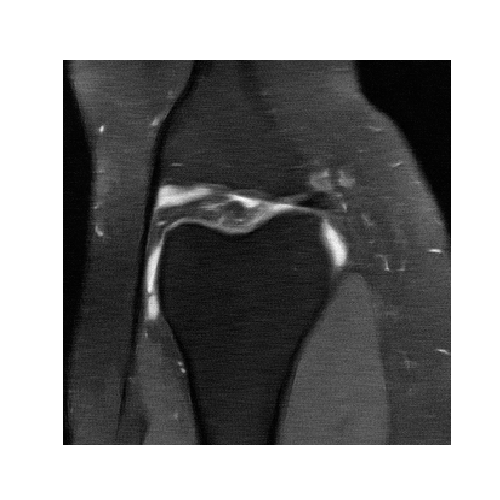
\includegraphics[width=\thefigdim\linewidth]{Figures/dl_mri_figures/bench_figs/kikinet-sep-16_recon_af4.png}&
        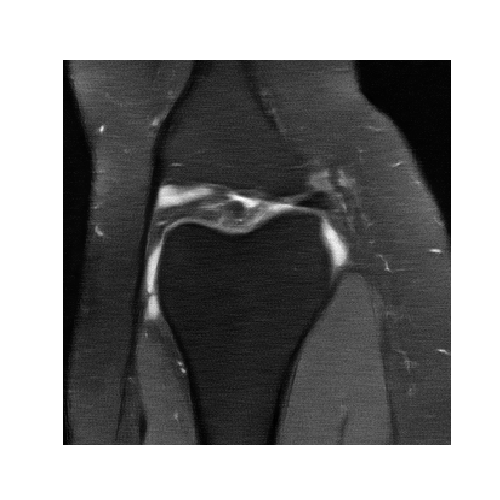
\includegraphics[width=\thefigdim\linewidth]{Figures/dl_mri_figures/bench_figs/unet_recon_af4.png}&
        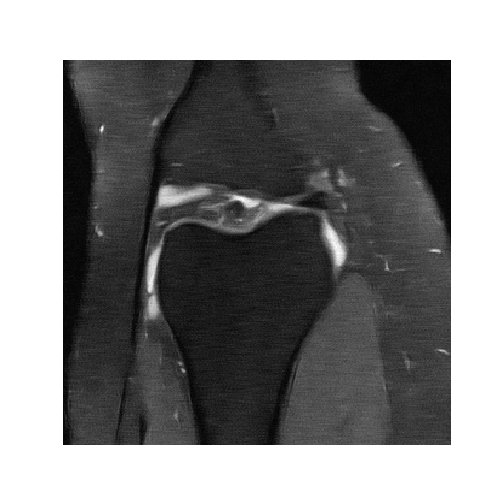
\includegraphics[width=\thefigdim\linewidth]{Figures/dl_mri_figures/bench_figs/cascadenet_recon_af4.png}&
        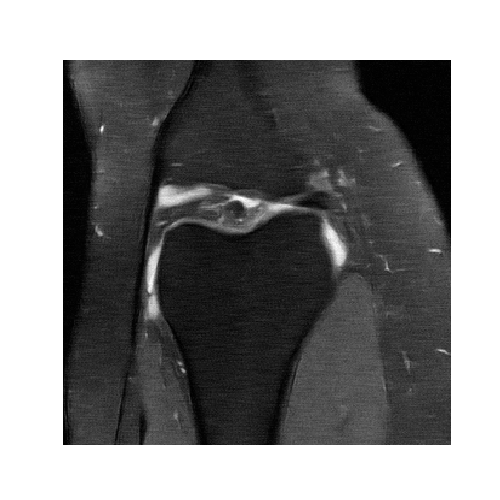
\includegraphics[width=\thefigdim\linewidth]{Figures/dl_mri_figures/bench_figs/pdnet_recon_af4.png}\\[-.70cm]
        &
        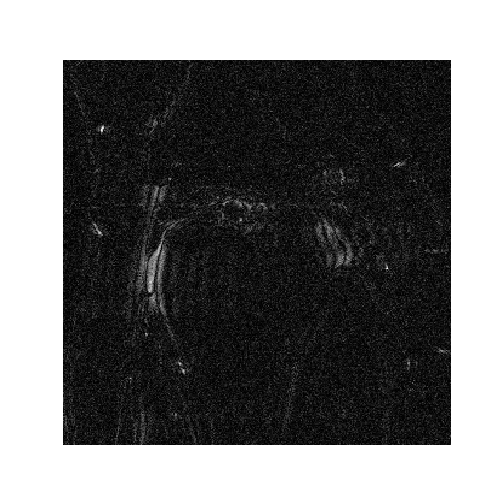
\includegraphics[width=\thefigdim\linewidth]{Figures/dl_mri_figures/bench_figs/zfilled_residu_af4.png}&
        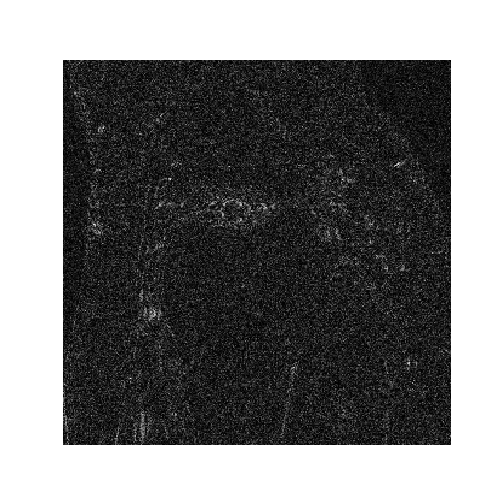
\includegraphics[width=\thefigdim\linewidth]{Figures/dl_mri_figures/bench_figs/kikinet-sep-16_residu_af4.png}&
        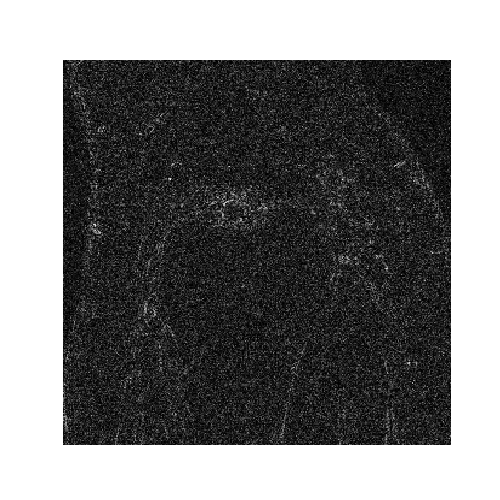
\includegraphics[width=\thefigdim\linewidth]{Figures/dl_mri_figures/bench_figs/unet_residu_af4.png}&
        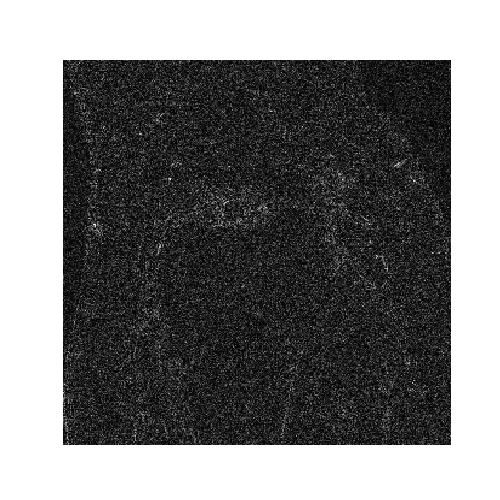
\includegraphics[width=\thefigdim\linewidth]{Figures/dl_mri_figures/bench_figs/cascadenet_residu_af4.png}&
        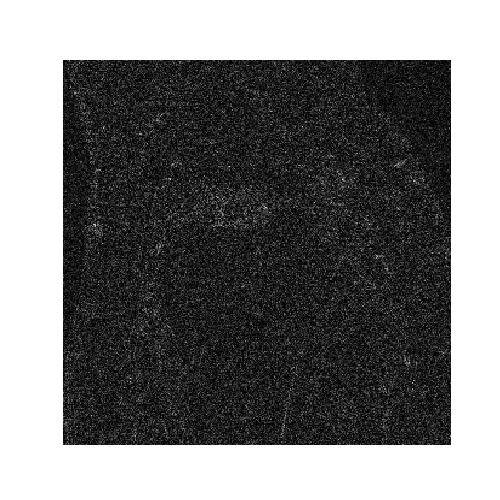
\includegraphics[width=\thefigdim\linewidth]{Figures/dl_mri_figures/bench_figs/pdnet_residu_af4.png}
        \end{tabular}
        \end{center}
        \end{figure}
\end{frame}


\begin{frame}{Unrolled models - 2}
    % first benchmark: different unrolling strategies give different results
    \begin{exampleblock}{Contribution \#1}
        \fullcite{Ramzi2020_benchmark_journal}
    \end{exampleblock}
    % We can build different models depending on the optimization algorithm we unroll, the choice of $f_{\thetab}$ and the number of iterations.
    Different models based on:
    \begin{itemize}
        \item optimization algorithm to unroll
        \item choice of $f_{\thetab}$
        \item $N$
    \end{itemize}


    \noindent\rule{\textwidth}{1pt}

        \begin{itemize}
            \item \faicon{github} Code available online: \texttt{github.com/zaccharieramzi/fastmri-reproducible-benchmark}
            \item\begin{tabular}{@{}c@{}}
\includegraphics[width=3ex]{Figures/hf_logo.jpeg}\end{tabular}Model weights available online: \texttt{huggingface.co/zaccharieramzi}
        \end{itemize}



\end{frame}

\begin{frame}{XPDNet}

\end{frame}

\begin{frame}{XPDNet}
    % talk about XPDNet archi
    \begin{center}
        \begin{tikzpicture}[
            font=\Large, node distance=1.5em,>=stealth,
            ionode/.style={rounded rectangle, draw=red!87, fill=red!17},
            unitnode/.style={rounded rectangle, draw=black!87, fill=black!7},
            opnode/.style={rounded rectangle, draw=green!87, fill=green!17},
            kspace_node/.style={rounded rectangle, draw=yellow!87, fill=yellow!17},
            image_node/.style={rounded rectangle, draw=blue!87, fill=blue!17},
            highlight_node/.style={rectangle, draw=red!70, dashed, inner sep=0.1em},
        ]
            % Unrolled net simple
            \node (input) {$\xb_0$};
            \only<1-2>{
                % nodes
                \node (first_unit) [fit=(dc_1)(prox_1), unitnode, inner sep=0.7em, visible on=<2>] {};
                \node (t_first_unit) [below right, visible on=<2>] at ($(first_unit.north west)+(-0.9em,0.25em)$) {\tiny Iteration Unit~(IU)};
                \node (second_unit) [fit=(dc_2)(prox_2), unitnode, inner sep=0.5em, visible on=<2>] {};
                \node (input) {$\xb_0$};
                \node (dc_1) [right=of input, kspace_node] {DC};
                \node (prox_1) [right=of dc_1, image_node] {$f_{\thetab_1}$};
                \node (dots) [right=of prox_1] {$\ldots$};
                \node (dc_2) [right=of dots, kspace_node] {DC};
                \node (prox_2) [right=of dc_2, image_node] {$f_{\thetab_N}$};
                \node (output) [right=of prox_2] {$\xb_{N}$};
                % arrows linking all nodes
                \draw [->] (input) -- (dc_1);
                \draw [->] (dc_1) -- (prox_1);
                \draw [->] (prox_1) -- (dots);
                \draw [->] (dots) -- (dc_2);
                \draw [->] (dc_2) -- (prox_2);
                \draw [->] (prox_2) -- (output);
            }
            % Unrolled net exploded
            \only<3->{
                % nodes
                %% main track
                \node (first_unit) [unitnode, right=of input] {IU};
                \node (dots) [right=of first_unit] {$\ldots$};
                \node (second_unit) [unitnode, right=of dots] {IU};
                \node (output) [right=of second_unit] {$\xb_{N}$};
                %% IU track
                %% applies \mathcal{A} (in green), then removes \ybb (in yellow), then applies \epsilon_1 \mathcal{A}^H (in green)
                %% then residual connection , then applies f_{\thetab_1} (in blue)
                \node (forward_op) [opnode, below=4em of first_unit] {$\mathcal{A} \cdot$};
                \node (input_forward) [left=3em of forward_op] {};
                \node (input_str_forward) [left=of input_forward] {$\xb_0$};
                \node (dc) [kspace_node, above right=of forward_op] {$\cdot - \ybb$};
                \node (backward_op) [opnode, right=of dc, visible on=<3>] {$\epsilon_1 \mathcal{A}^H \cdot$};
                \node (simple_backward_op) [opnode, right=of dc, visible on=<4->] {$\mathcal{A}^H \cdot$};
                \node (dc_res) [rounded rectangle, draw, fill=white, below right=of backward_op, visible on=<3>] {$-$};
                \node (dc_concat) [rounded rectangle, draw, fill=white, below right=of backward_op, visible on=<4->] {$\operatorname{concat}$};
                \node (prox) [image_node, right=of dc_concat] {$f_{\thetab_1}$};
                \node (prox_exp_cnn) [below=2em of prox, visible on=<3-4>] {CNN};
                \node (prox_exp_mwcnn) [below=2em of prox, visible on=<5->] {MWCNN\footfullcite{Liu2018}};
                \node (outpt_prox) [right=3em of prox] {$\xb_1$};
                % smaps nodes
                \node (smaps_refiner) [opnode, below left=of forward_op, visible on=<6->] {Smaps refiner\footfullcite{Sriram2020End-to-EndReconstruction}};
                \node (smaps) [left=of smaps_refiner, visible on=<6->] {$\Sbb$};
                \node (smaps_exp) [below=0.4em of smaps_refiner, visible on=<6->] {U-Net\footfullcite{ronneberger2015u}};
                \begin{scope}[on background layer]
                    \node (encompassing_unit) [unitnode, fit=(forward_op)(dc)(simple_backward_op)(backward_op)(dc_concat)(dc_res)(prox), inner sep=0.9em] {};
                    %% highlighting nodes
                    \node (highlight_concat) [highlight_node, fit=(backward_op) (dc_concat), visible on=<4>] {};
                    \node (highlight_mwcnn) [highlight_node, fit=(prox_exp_mwcnn), visible on=<5>] {};
                    \node (highlight_smaps) [highlight_node, fit=(smaps_refiner) (smaps) (smaps_exp), visible on=<6>] {};
                \end{scope}
                % arrows linking all nodes
                %% main track
                \draw [->] (input) -- (first_unit);
                \draw [->] (first_unit) -- (dots);
                \draw [->] (dots) -- (second_unit);
                \draw [->] (second_unit) -- (output);
                %% IU track
                \draw [->] (input_forward) -- (forward_op);
                \draw [->] (forward_op) -| (dc);
                \draw<3> [->] (dc) -- (backward_op);
                \draw<4-> [->] (dc) -- (simple_backward_op);
                \draw<3> [->] (backward_op) -| (dc_res);
                \draw<4-> [->] (simple_backward_op) -| (dc_concat);
                \draw<3> [->] plot [smooth, tension=0.7] coordinates{(input_forward.east)  ($(forward_op.south)+(0, -0.6em)$) (dc_res.west)};
                \draw<4-> [->] plot [smooth, tension=0.7] coordinates{(input_forward.east)  ($(forward_op.south)+(0, -0.6em)$) (dc_concat.west)};
                \draw (input_str_forward) -- (input_forward.east);
                \draw<3> [->] (dc_res) -- (prox);
                \draw<4-> [->] (dc_concat) -- (prox);
                \draw [->] (prox) -- (outpt_prox);
                \draw [line width=0.1em] (first_unit.south) -- (encompassing_unit.north west);
                \draw<3-4> [line width=0.1em] (prox.south) -- (prox_exp_cnn.north);
                \draw<5-> [line width=0.1em] (prox.south) -- (prox_exp_mwcnn.north);
                % smaps arrows
                \draw<6-> [<-] (smaps_refiner) -- (smaps);
                \draw<6-> [->] (smaps_refiner) -| (forward_op);
                \draw<6-> [->] (smaps_refiner) -| (simple_backward_op);
                \draw<6-> [line width=0.1em] (smaps_refiner.south) -- (smaps_exp.north);
            }

        \end{tikzpicture}
    \end{center}
\end{frame}

\begin{frame}{fastMRI challenge}
    % mention fastMRI challenge results
    \begin{exampleblock}{Contributions \#2}
        \begin{itemize}
            \item \fullcite{Muckley2021}
            \item \fullcite{Ramzi2020_xpdnet}
        \end{itemize}
    \end{exampleblock}

    \begin{overprint}

        \onslide<2>
        \noindent\rule{\textwidth}{1pt}

        \begin{itemize}
            \item Data: fastMRI
            \item Compute: Jean Zay
        \end{itemize}

        \onslide<3>
        \begin{table}[]
            \centering
            \caption{\textbf{fastMRI challenge radiologist evaluation.}}
            \label{tab:fastmri-challenge}
            \begin{tabular}{|l|c|c|}
            \hline
            \textbf{Team}      & \textbf{Rank 4X} & \textbf{Rank 8X} \\ \hline
            \textbf{AIRS}      & 1.36             & 1.28             \\ \hline
            \highlight{blue}{\textbf{NeuroSpin}} & 1.94             & 2.25             \\ \hline
            \textbf{ATB}       & 2.22             & 2.28             \\ \hline
            \end{tabular}
        \end{table}
    \end{overprint}
\end{frame}


\begin{frame}
    \def\thefigdimigogd{.35}

    \hspace*{-.7cm}
    \begin{tabular}{c@{\hspace*{\qualifigsepigogd}}c@{\hspace*{\qualifigsepigogd}}c}
        {\textbf{Reference}} & \makecell{{\textbf{GRAPPA }} \\ PSNR: 26, SSIM: 0.77} & \makecell{{\textbf{XPDNet}} \\ PSNR: 36, SSIM: 0.96} \\
        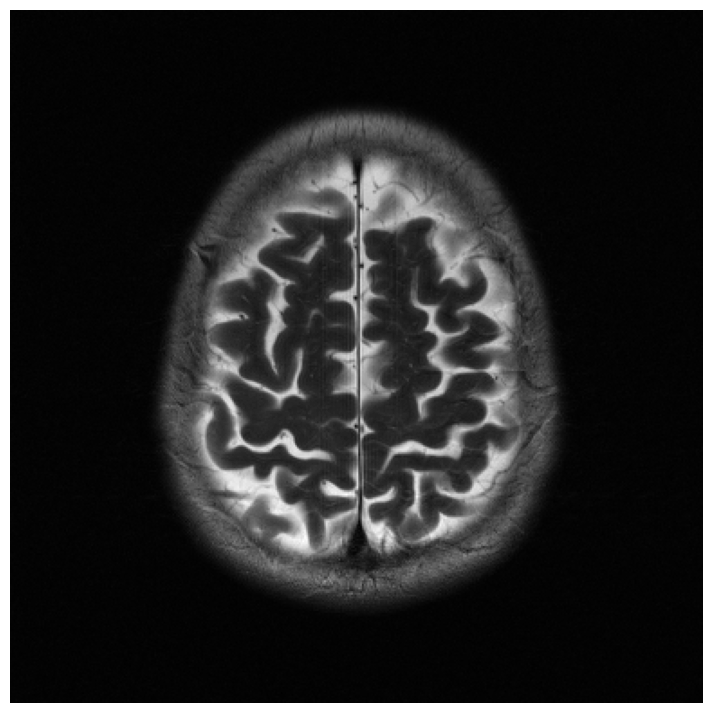
\includegraphics[width=\thefigdimigogd\textwidth]{Figures/clinic_applic/fastmri_r8/GT_Pinf_S1.0000.png}&
        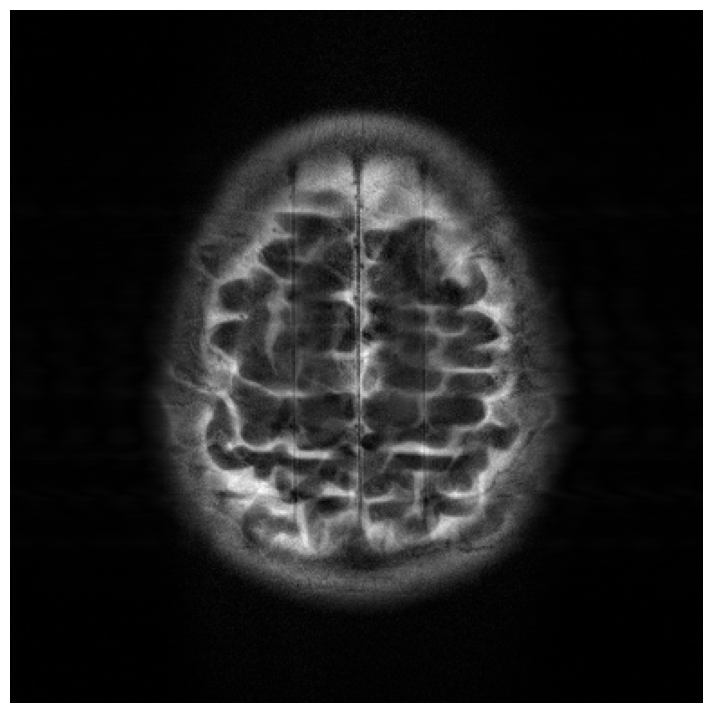
\includegraphics[width=\thefigdimigogd\textwidth]{Figures/clinic_applic/fastmri_r8/GRAPPA-ideal_P26.18_S0.7704.png}&
        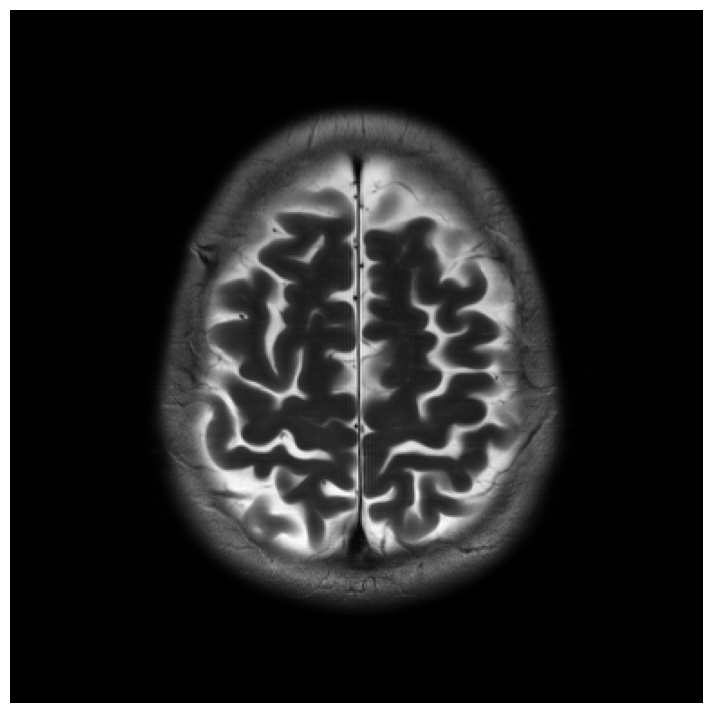
\includegraphics[width=\thefigdimigogd\textwidth]{Figures/clinic_applic/fastmri_r8/NN_P36.82_S0.9626.png}
    \end{tabular}

\end{frame}

\begin{frame}{Robustness test}
    % XXX: only if we decide not to have clinical applicability
    % How does the XPDNet fare in a prospective out-of-distribution setting:
    XPDNet in a prospective out-of-distribution setting:\footfullcite{Marrakchi-Kacem2016RobustChoices}

    different orientation, higher resolution, higher field strength, lower acceleration factor, presence of the cerebellum.\footnote{For anonymity reasons, the cerebellum is not present in the fastMRI dataset.}

\end{frame}

\begin{frame}
    \begin{figure}[h]
        \begin{center}
        \begin{tabular}{c@{\hspace*{\qualifigsepigogd}}c}
        {\textbf{GRAPPA }} & {\textbf{XPDNet}} \\
        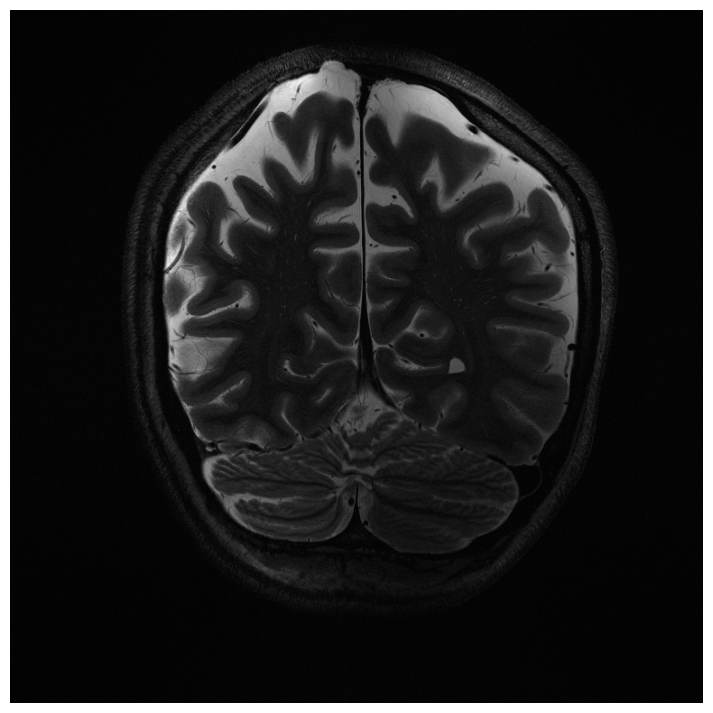
\includegraphics[width=0.38\textwidth]{Figures/clinic_applic/gt_brain_7t.png}&
        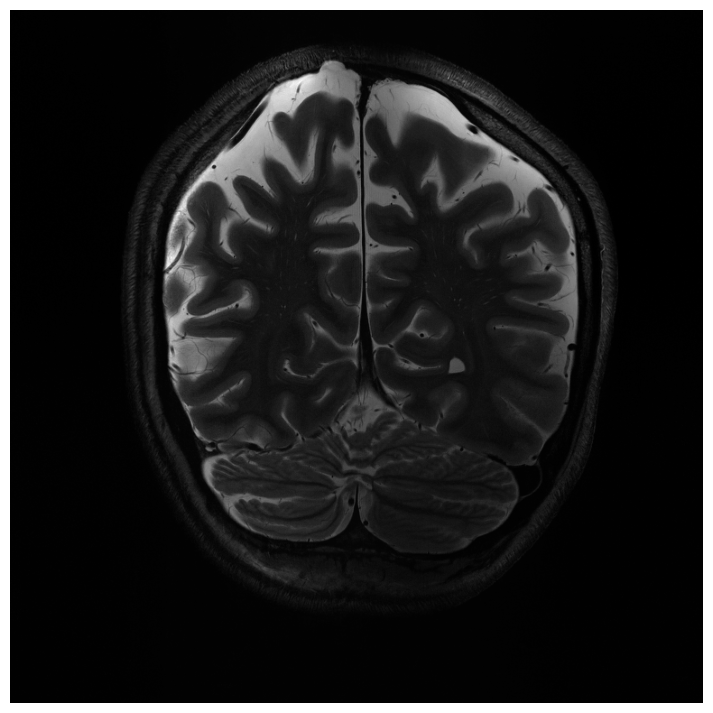
\includegraphics[width=0.38\textwidth]{Figures/clinic_applic/brain_nn_recon.png}\\
        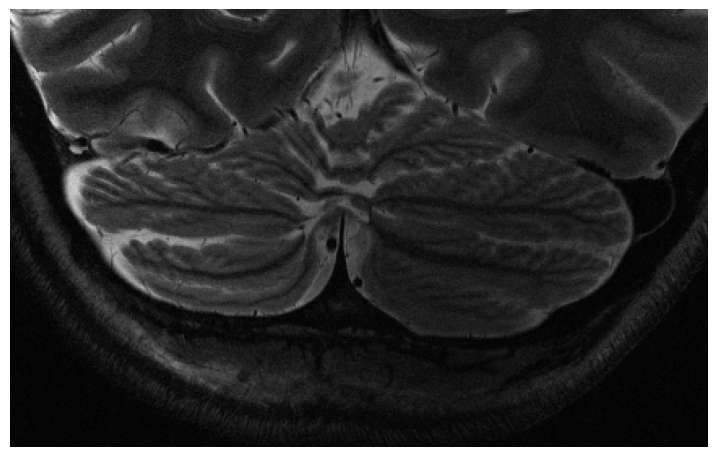
\includegraphics[width=0.38\textwidth]{Figures/clinic_applic/gt_brain_7t_zoom.png}&
        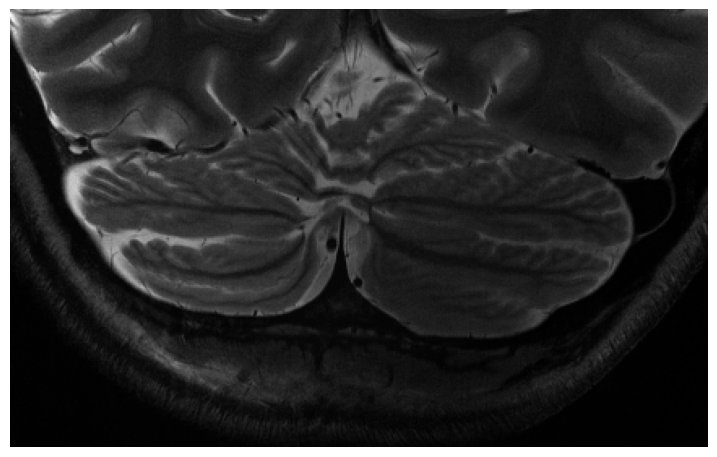
\includegraphics[width=0.38\textwidth]{Figures/clinic_applic/brain_nn_recon_zoom.png}
        \end{tabular}
        \caption{\textbf{XPDNet reconstruction on a brain prospectively accelerated.} (zoom on the cerebellum) \label{fig:brain-7t}}
        \end{center}
        \end{figure}
\end{frame}

\begin{frame}{Non-Cartesian acquisitions}
    % Why do we need non-Cartesian acquisitions?
    % We need non-Cartesian acquisitions to better cover the k-space.
    Non-Cartesian acquisitions better cover the k-space.
    \pause
    \vspace{-1ex}
    \begin{figure}
        \centering
        \begin{subfigure}{0.48\textwidth}
            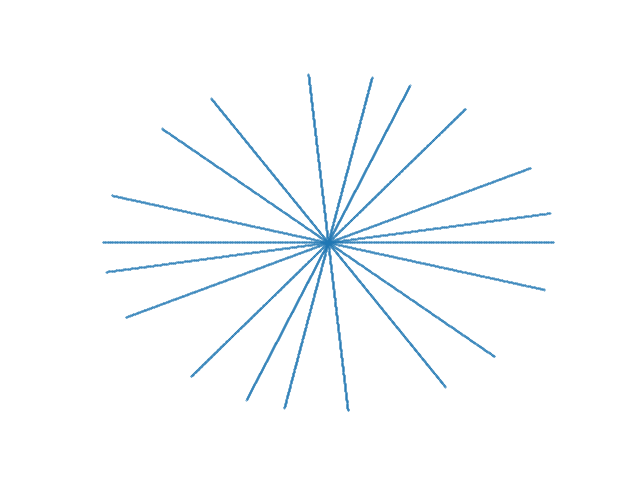
\includegraphics[height=0.48\textheight]{Figures/dl_mri_figures/radial_trajectory.png}
        \end{subfigure}
        \begin{subfigure}{0.48\textwidth}
            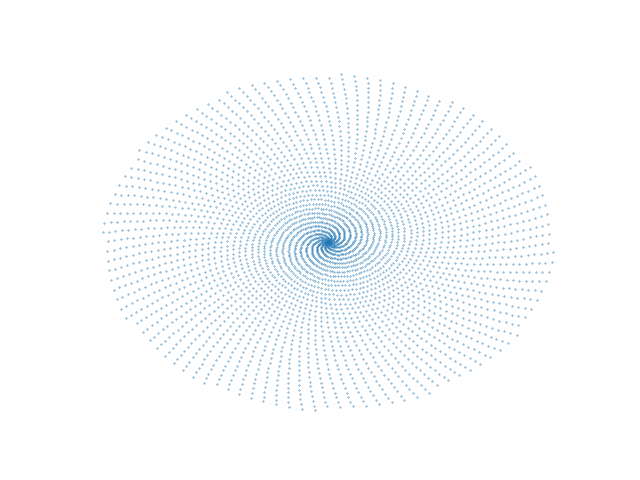
\includegraphics[height=0.48\textheight]{Figures/dl_mri_figures/spiral_trajectory.png}
        \end{subfigure}
        \caption{\textbf{Radial and spiral undersampled trajectories.}}
    \end{figure}
    \pause

    % The difficulty from a computational point of view is that we need to now use the \textbf{Nonuniform Fourier Transform (NDFT)}.
    \textbf{Nonuniform Fourier Transform (NDFT)} too costly $\Rightarrow$ NUFFT, with the TensorFlow implementation:
    % We resort to using its fast approximation, the NUFFT, which we implemented in TensorFlow, to enable gradient-based learning:
    \begin{itemize}
        \item \faicon{github} Code available online: \texttt{github.com/zaccharieramzi/tfkbnufft}
    \end{itemize}
\end{frame}

\begin{frame}{NC-PDNet - 1}
    % explain NC-PDNet and density compensation
    \begin{center}
        \begin{tikzpicture}[
            font=\Large, node distance=1em,>=stealth,
            ionode/.style={rounded rectangle, draw=red!87, fill=red!17},
            unitnode/.style={rounded rectangle, draw=black!87, fill=black!7},
            opnode/.style={rounded rectangle, draw=green!87, fill=green!17},
            kspace_node/.style={rounded rectangle, draw=yellow!87, fill=yellow!17},
            image_node/.style={rounded rectangle, draw=blue!87, fill=blue!17},
            highlight_node/.style={rectangle, draw=red!70, dashed, inner sep=0.1em},
        ]
            % Unrolled net simple
            \node (input) {$\xb_0$};
            % Unrolled net exploded
            % nodes
            %% main track
            \node (first_unit) [unitnode, right=of input] {IU};
            \node (dots) [right=of first_unit] {$\ldots$};
            \node (second_unit) [unitnode, right=of dots] {IU};
            \node (output) [right=of second_unit] {$\xb_{N}$};
            %% IU track
            %% applies \mathcal{A} (in green), then removes \ybb (in yellow), then applies \epsilon_1 \mathcal{A}^H (in green)
            %% then residual connection , then applies f_{\thetab_1} (in blue)
            \node (forward_op) [opnode, below=4em of first_unit] {$\mathcal{A} \cdot$};
            \node (input_forward) [left=3em of forward_op] {};
            \node (input_str_forward) [left=of input_forward] {$\xb_0$};
            \node (dc) [kspace_node, above right=of forward_op] {$\cdot - \ybb$};
            \node (dcp) [kspace_node, right=of dc, visible on=<2->] {$\cdot \times$ DCp\footfullcite{Pipe1999SamplingSolution}};
            \node (backward_op) [opnode, right=of dcp] {$\mathcal{A}^H \cdot$};
            \node (dc_input_comb) [rounded rectangle, draw, fill=white, below right=of backward_op] {$\operatorname{concat}$};
            \node (prox) [image_node, right=of dc_input_comb] {$f_{\thetab_1}$};
            \node (prox_exp) [below=2em of prox] {CNN};
            \node (outpt_prox) [right=3em of prox] {$\xb_1$};
            \begin{scope}[on background layer]
                \node (encompassing_unit) [unitnode, fit=(forward_op)(dc)(backward_op)(dc_input_comb)(prox), inner sep=0.9em] {};
                \node (t_first_unit) [below right] at ($(encompassing_unit.north west)+(-0.9em,0.25em)$) {\tiny Iteration Unit};
            \end{scope}
            %% smaps nodes
            \node (smaps_refiner) [opnode, below left=1.5em of forward_op] {Smaps refiner};
            \node (smaps) [left=of smaps_refiner] {$\Sbb$};
            %% highlight nodes
            \node<2> (highlight_dcp) [highlight_node, fit=(dcp)] {};
            % arrows linking all nodes
            %% main track
            \draw [->] (input) -- (first_unit);
            \draw [->] (first_unit) -- (dots);
            \draw [->] (dots) -- (second_unit);
            \draw [->] (second_unit) -- (output);
            %% IU track
            \draw [->] (input_forward) -- (forward_op);
            \draw [->] (forward_op) -| (dc);
            \draw<2-> [->] (dc) -- (dcp);
            \draw<2-> [->] (dcp) -- (backward_op);
            \draw<1> [->] (dc) -- (backward_op);
            \draw [->] (backward_op) -| (dc_input_comb);
            \draw [->] plot [smooth, tension=0.7] coordinates{(input_forward.east) ($(forward_op.south)+(0, -0.6em)$) (dc_input_comb.west)};
            \draw (input_str_forward) -- (input_forward.east);
            \draw [->] (dc_input_comb) -- (prox);
            \draw [->] (prox) -- (outpt_prox);
            \draw [line width=0.1em] (first_unit.south) -- (encompassing_unit.north west);
            \draw [line width=0.1em] (prox.south) -- (prox_exp.north);
            % smaps arrows
            \draw [<-] (smaps_refiner) -- (smaps);
            \draw [->] (smaps_refiner) -| (forward_op);
            \draw [->] (smaps_refiner) -| (backward_op);

        \end{tikzpicture}
    \end{center}
\end{frame}

\begin{frame}{NC-PDNet - 2}
    % give results
    \begin{exampleblock}{Contribution \#3}
        \fullcite{Ramzi2021_ncpdnet_journal}
    \end{exampleblock}


\end{frame}

\begin{frame}
    \begin{figure}
        \begin{overprint}
            \onslide<1>\centering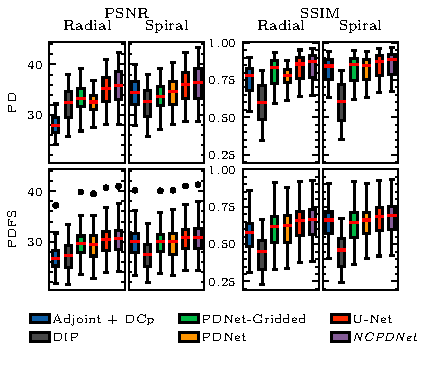
\includegraphics[height=0.9\textheight]{Figures/dl_mri_figures/single_coil.pdf}\caption{\textbf{2D single-coil reconstruction quantitative results on the fastMRI knee dataset.}}
            \onslide<2>\centering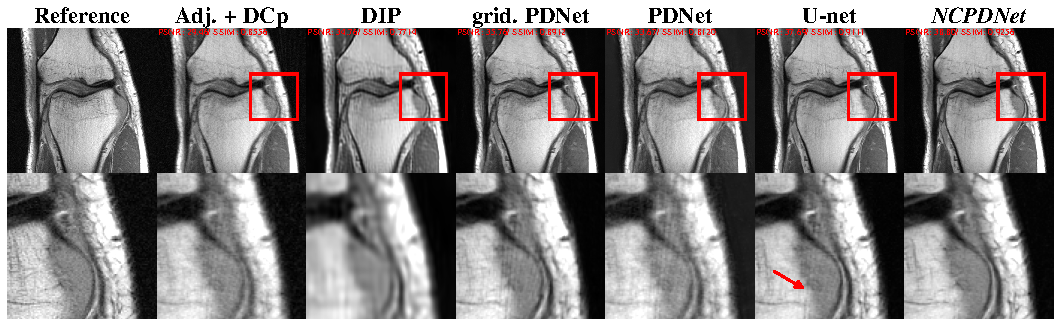
\includegraphics[width=\textwidth]{Figures/dl_mri_figures/quali_no_err_af4_radial.pdf}\caption{\textbf{2D single-coil reconstruction qualitative results on the fastMRI dataset for a radial trajectory.}}
            \onslide<3>\centering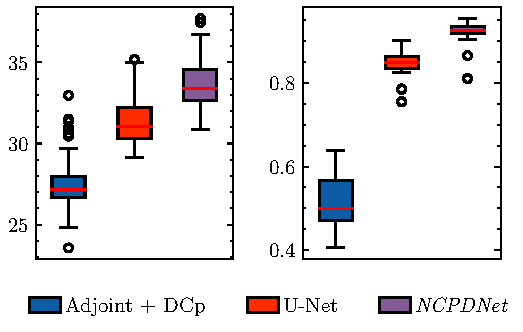
\includegraphics[width=0.7\textwidth]{Figures/dl_mri_figures/3d.pdf}\caption{\textbf{3D single-coil reconstruction quantitative results on the OASIS dataset for a radial trajectory.}}
            \onslide<4>\centering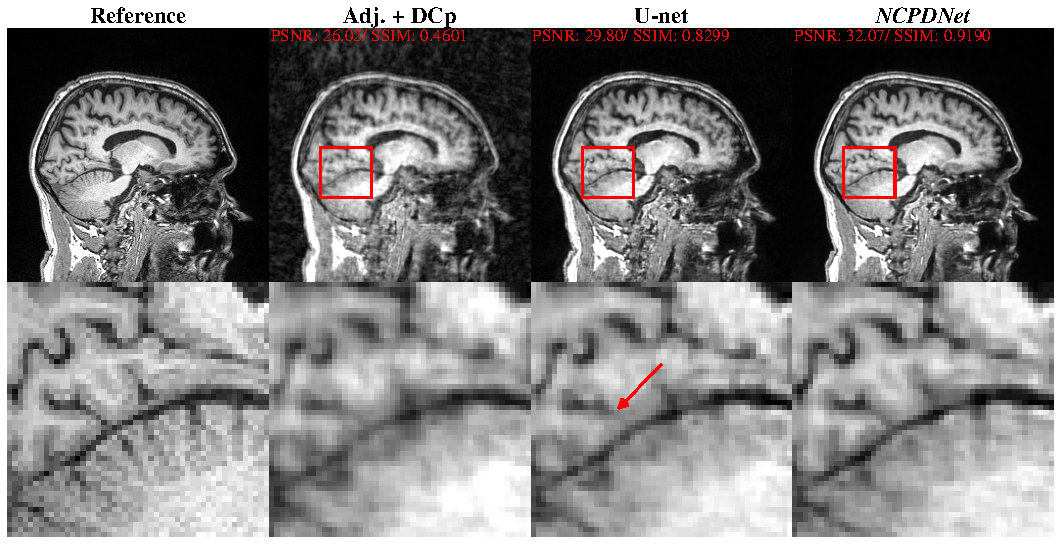
\includegraphics[width=\textwidth]{Figures/dl_mri_figures/quali_no_err_3d_af4_radial.pdf}\caption{\textbf{3D single-coil reconstruction qualitative results on the OASIS dataset for a radial trajectory.}}
        \end{overprint}
    \end{figure}
\end{frame}

\begin{frame}{Unrolled models for MRI reconstruction}
    % cool: we are starting to have good results, let's not forget the end goal
    % use this in a scanner so that the MRI exam is faster
    % how will this technique fare in the clinical setting ? <This would be in the case of using clinical applic chapther>
    % <otherwise>: ok we get good results, but we have sacrificed a bit of power in 3D, and multi-coil is not possible as is
    \begin{block}{Recap}
        MRI is slow because of \textbf{relaxation}.

        \pause
        If we want to do fewer relaxations, we need to exploit some \textbf{redundancy} in MR images.

        \pause
        \textbf{Deep Learning} allows us to learn more complex structures in MR images than Compressed Sensing.
        We showcased 2 instances of unrolled models, \textbf{XPDNet} and \textbf{NC-PDNet}, which can perform really well in challenging acquisition settings.
    \end{block}

    \pause
    But we needed to trade off some model capacity for memory, in order to train the models in the 3D single-coil case.
    How will this fare going to 3D multi-coil?
\end{frame}